\section{Trigonometric Functions}


\subsection{The Unit Circle}
\begin{frame}
    \frametitle{The Unit Circle}
\begin{definition}
    The \textbf{unit circle} is the circle in the Cartesian plane with center at the origin and radius 1, defined by the equation:
    \[
    x^2 + y^2 = 1
    \]
\end{definition}                                                                                                                                    
\end{frame}


 \begin{frame}
        \frametitle{Radius corresponding to a positive angle}
        \centering
        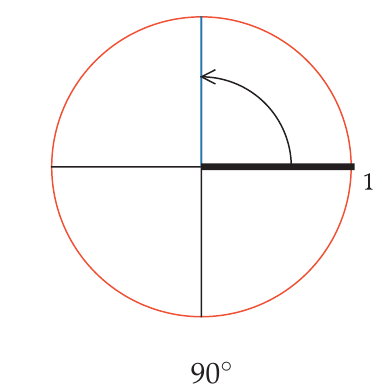
\includegraphics[scale=0.5]{/unit_circle/1.png}
    \end{frame}
    
    \begin{frame}
        \frametitle{Radius corresponding to a negative angle}
        \centering
        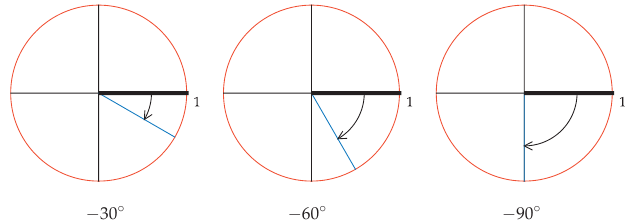
\includegraphics[scale=0.5]{/unit_circle/2.png}

    \end{frame}
    
    \begin{frame}
        \begin{block}{Positive and Negative Angles}
            \begin{itemize}
                \item Angle measurements for a radius on the unit circle are made from the
                positive horizontal axis.
                \item Positive angles correspond to moving counterclockwise from the positive
                horizontal axis.
                \item Negative angles correspond to moving clockwise from the positive hori-
                zontal axis.
            \end{itemize}
        \end{block}
    \end{frame}
    
    \begin{frame}
        \frametitle{Angles more than 360 degrees}
    \begin{block}{cyclic behaviour of angles}
        A radius of the unit circle corresponding to $\theta$ degrees also corresponds to
    $\theta + 360n$ degrees for every integer n.
    \end{block}
        \begin{figure}[h]    
            \centering
            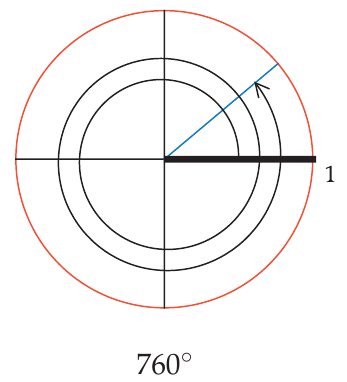
\includegraphics[scale=0.4]{/unit_circle/3.png}
        \end{figure}
        
    \end{frame}
    


    \begin{frame}
        \frametitle{Length of a Circular Arc}
        \begin{figure}
            \centering
            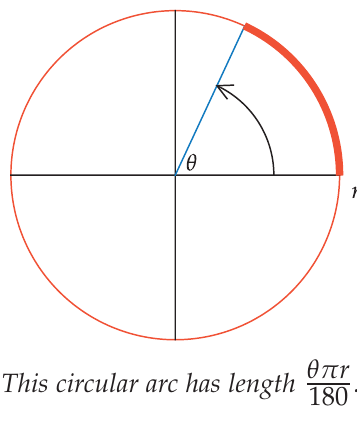
\includegraphics[scale=0.5]{/unit_circle/5.png}
        \end{figure}
        \[ 360^{\circ}   \rightarrow  2 \pi r \implies \theta^{\circ}  \rightarrow \frac{\theta}{360}.2\pi r  = \frac{\theta \pi r}{180}\] 
    \end{frame}
    
    \begin{frame}
        \frametitle{Radians}
        For example an ant moving around a unit circle would travel a distance of $2\pi$ radians
        when it completes one full rotation.
       \begin{block}{Radians}
        Radians are a unit of measurement for angles such that $2\pi$ radians correspond
        to a rotation through an entire circle.
       \end{block}
    \end{frame}
    

    \begin{frame}
        \frametitle{Radians}
       \begin{block}{Degree to Radians}
    
        \[ 360^{\circ} = 2 \pi \text{ radians} \]
        \[ \theta ^{\circ}  = \frac{\theta \pi}{180} \text{ radians} \]
        
       \end{block}
    \end{frame}
    
    \begin{frame}
        \frametitle{Arc Length}
        \begin{block}{length of a circular arc}
            If $0 < \theta \leq 2\pi$ , then a circular arc on the unit circle corresponding to $\theta$ radians
            has length $\theta$         
        \end{block}
    \end{frame}

    \begin{frame}
        \frametitle{Area of a Sector}
        \begin{block}{Area of a sector}
            A sector/slice with angle $\theta$ radians inside a circle with radius $r$ has area $\frac{1}{2} \theta r^{2}$ .
        \end{block}
        \begin{figure}[h]    
            \centering
            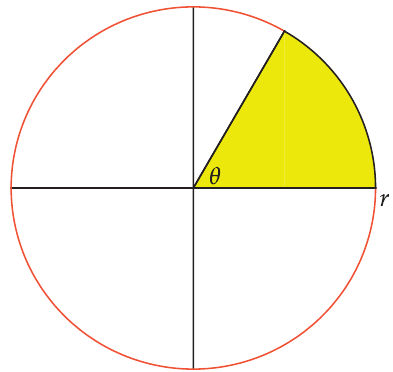
\includegraphics[scale=0.25]{unit_circle/6.png}
        \end{figure}
    \end{frame}
    
    \begin{frame}
        \frametitle{Note}
        \begin{block}{Note}
            If no unit is specified, angles are assumed to be in radians.
        \end{block}
    \end{frame}

    \begin{frame}
        \frametitle{Cosine and Sine}
        \begin{block}{Definitions}
            \begin{itemize}
                \item The \textbf{cosine} of an angle $\theta$ is the x-coordinate of the point on the unit circle corresponding to that angle.
                \item The \textbf{sine} of an angle $\theta$ is the y-coordinate of the point on the unit circle corresponding to that angle.
            \end{itemize}
        \end{block}     
        \begin{figure}[h]    
            \begin{minipage}[b]{0.8\textwidth}
            \centering
            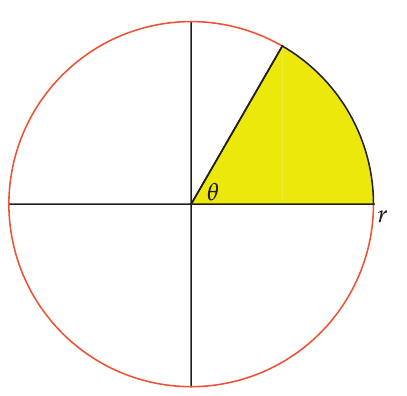
\includegraphics[scale=0.22]{unit_circle/7.png}
            \caption{sine and cosine}
        \end{minipage}
    \end{figure}
    \end{frame}

    \begin{frame}
        \frametitle{The Signs of Sine and Cosine} 
        \begin{figure}
            \centering
            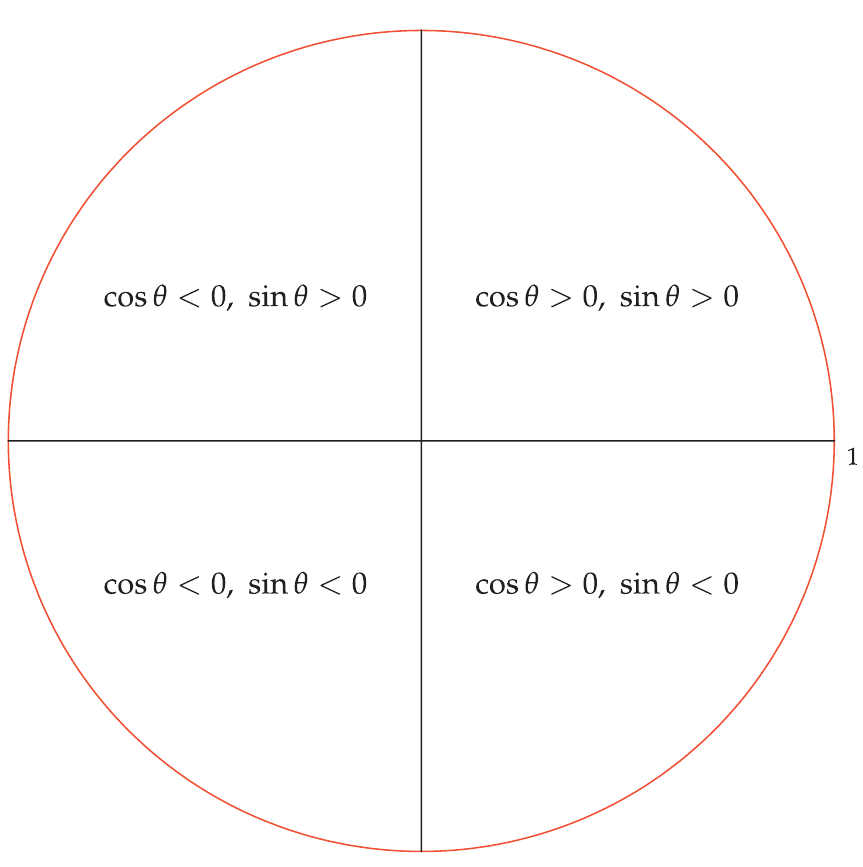
\includegraphics[scale=0.2]{unit_circle/8.png}
            \caption{Signs of sine and cosine in different quadrants}
        \end{figure}
    \end{frame}

    \begin{frame}
        \frametitle{Key Equation Connecting Sine and Cosine} 
        \begin{itemize}
            \item By definition cosine and sine are the x and y coordinates of a point on the unit circle.
            \item The equation of the unit circle is $x^2 + y^2 = 1$.
            \item Therefore, for any angle $\theta$,
        \end{itemize}
        \begin{block}{Key Identity}
            \[\cos^2(\theta) + \sin^2(\theta) = 1\]
        \end{block}
    \end{frame}

    \begin{frame}
        \frametitle{The limits of Sine and Cosine} 
        \begin{itemize}
            \item For each real number $\theta$, there is a radius of the unit circle corresponding to that angle.
            \item The co-ordinates of the end point of the radius are $(\cos(\theta), \sin(\theta))$.
            \item That is this function is defined for all real numbers because theta can take any real value. 
            \item The domain of sine and cosine is all real numbers. \(\mathbb{R}\) 
            \item For unit circle \( \cos \theta^{2} + \sin \theta^{2} = 1 \) 
            \item Because \( \cos \theta^{2} + \sin \theta^{2} = 1 \) for all \(\theta\), the range of both sine and cosine is limited to \([-1, 1]\).
            \item 
        \end{itemize}
    \end{frame}
